\documentclass[a4paper, 11pt]{article}
\newcommand{\systemTitle}{NINSHIKI}
\usepackage[bottom]{footmisc}
\usepackage{minted}
\usepackage{graphicx}
\usepackage{hyperref}
\graphicspath{ {./Images/} }
\usepackage{fontspec}
    \setmainfont[Path = ./MavenPro/,
 				  Extension = .ttf,
 				  UprightFont = *-Regular,
 				  BoldFont = *-Bold]
                  {MavenPro}
    \setsansfont[Path = ./NunitoSans/,
 				  Extension = .ttf,
 				  UprightFont = *-Light,
 				  BoldFont = *-SemiBold,
                  ItalicFont = *-LightItalic]
                  {NunitoSans}
\usepackage{fancyhdr}
    \pagestyle{fancy}
    \fancyhf{}
    \rhead{Software Sharks}
    \setlength{\headheight}{16pt} 
    \lhead{\systemTitle{} - System Requirements & Design Document}
    \rfoot{Page \thepage}


\title{System Requirements & Design Document}
\author{Software Sharks}
\date{September 2018}

\begin{document}

%----------------------------------------------------------------------------------------
%	TITLE PAGE
%----------------------------------------------------------------------------------------
\begin{titlepage}
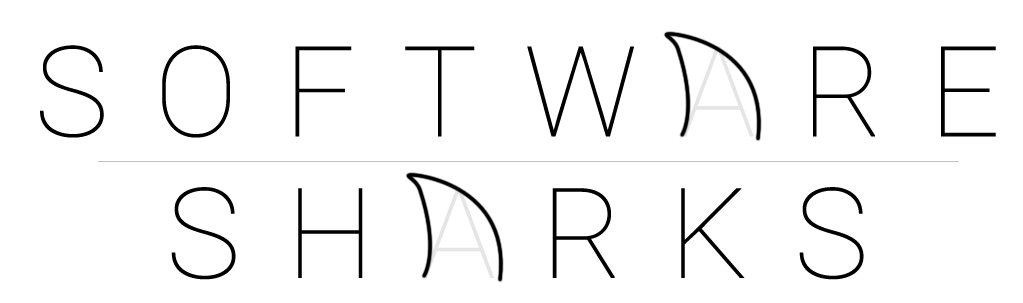
\includegraphics[width=0.5\linewidth]{Images/sslogo.png}
	\centering
	
    \scshape
    \sffamily
	
	\vspace*{\baselineskip}
	
	\rule{\textwidth}{3pt}
	
	\vspace{0.75\baselineskip}
	
	\textrm{\LARGE \textbf{System Requirements \& Design Document} \\ for\\ \systemTitle{}\\ \small Version 1.0.0 - Demo \#5 Final\\}
	
	\vspace{0.75\baselineskip}
	
	\rule{\textwidth}{3pt} 
	
	\vspace{2\baselineskip}
% 	TO-DO: Change to relevant description of SRS Document purpose/contents
	A document providing an overview of the Ninshiki system, a specification of the system requirements, and the architectural design of the system.\\
	
	\vspace*{3\baselineskip}
	
	Compiled By
	
	\vspace{0.5\baselineskip}
	
    \textsf{\large
    \textrm{\textbf{The Software Sharks Team}} \\
    \small 
    Coetzer MJ \\
    Bester TJ \\
    Orrie O \\
    Lew J \\
    Matodzi MC \\
    } 
	
	\vspace{0.5\baselineskip}
	
	\textit{ Department of Computer Science \\ The University of Pretoria}
	
    \vfill
    
    \includegraphics[width=0.5\linewidth]{Images/uplogo.png}
    \vfill
    For
	
	\vspace{0.5\baselineskip}
	
    \textsf{\large
    \textrm{\textbf{Bramhope International School of Innovation}} \\
    } 

\end{titlepage}

\pagebreak

%----------------------------------------------------------------------------------------
%	COPYRIGHT PAGE
%----------------------------------------------------------------------------------------

\newpage
~\vfill
\thispagestyle{empty}

\noindent COS 301 Team: Software Sharks\\ 

\noindent \textsc{Department of Computer Science, University of Pretoria}\\

\noindent \textsc{https://github.com/OrishaOrrie/SoftwareSharks}\\ % URL \linebreak
\linebreak
% TO-DO: Change to SRS specifics
\noindent This Systems Requirements and Design document was drafted under the supervision of involved lecturers according to the assessment guidelines of the final year Computer Science module: COS 301 - Software Engineering, presented by the Department of Computer Science in the faculty of Engineering, Built Environment and Information Technology at the University of Pretoria during the first and second semester of the year 2018. \\ \\

\noindent \textit{First release, September 2018} % Edition date

\pagebreak
%----------------------------------------------------------------------------------------
%	Table of Contents
%----------------------------------------------------------------------------------------
\tableofcontents

\pagebreak
%----------------------------------------------------------------------------------------
%	Introduction
%----------------------------------------------------------------------------------------
\section{Introduction}
The purpose of this document is to provide a detailed description of the requirements for the Ninshiki image recognition system. It will explain the purpose, features and architectural design of the system, as well as system constraints. This document is intended to be proposed to University of Pretoria lecturers and the project owner, as well as a reference for developing the first version of the system.

%----------------------------------------------------------------------------------------
%	System Overview
%----------------------------------------------------------------------------------------
\section{System Overview}
The system’s main requirement and primary purpose is to enable a user to take an image of an object, compare the image to a predefined model, and have the application respond with a labeled classification of the object.
\linebreak
\linebreak
The system is made up of two core components, namely, the web application and the mobile application. From this point on in the document, the web application and mobile application will be referred to as “the application”, because both of these applications serve the same purpose and have similar interfaces with both the user and the back-end server.
\linebreak
\linebreak 
The user will make use of the application device (the device that is running the application) to capture an image of an object with a Webcam or mobile camera device. Then, using the designed interface, the user will be able to push the image to the application.
Once the application receives the image, the image gets processed by the image recognition model. After processing, the model outputs a prediction of the classification of the object. A list of the predictions is then created and returned to the user.
\subsection{Purpose}
% Justify the business need for the system
\begin{flushleft}
The objective of the project is to develop an interface that is capable of using image recognition technology to accurately identify a specific object within an image and then return a response with the object’s classification in the context of the client’s warehouse inventory.
\end{flushleft}

\pagebreak
\subsection{Project Scope}
% Explain the functionality of the system in broad terms.
\begin{flushleft}
Ninshiki is an image recognition app specifically intended to identify engineering supplies in a warehouse in order to help employees of a warehouse correctly stock the supplies. The system will be able to recognise images, learn from those images, allow users to request a quote as well as help employees with the counting of supplies. The system will be both web and mobile based. The website can be accessed through any browser while the app will only be available to download on a phone which runs on the Android operating system. 
\linebreak
\linebreak
The objective of the system is to help employees who are not familiar with engineering supplies to correctly stock the warehouse and add the supplies in the correct supply bins. This will benefit the warehouse as all supplies will be properly organised and employees will not waste time trying to figure out what the object is and where it belongs. 
\end{flushleft}

\subsection{Definitions, Acronyms and Abbreviations}
% Describe definitions, acronyms and abbreviations for the terminology used in the document.
\begin{itemize}
\item BISI : Bramhope International School Of Innovation
\item R\# : Requirements number
\item UC\# : Use Case number
\end{itemize}

\subsection{References}
IEEE Software Engineering Standards Committee, “IEEE Std 830-1998, IEEE Recommended
Practice for Software Requirements Specifications”, October 20, 1998.

\pagebreak
\subsection{UML Domain Model\protect\footnote{\href{https://drive.google.com/file/d/1LH17gMm1LskQkoO_7QEn8iQRw6mYI1KG/view?usp=sharing}{Complete Domain Model Diagram Link}}}
% Describe and model real world entities of your project and show the relationships between them, which collectively describe the problem domain space.
The domain model describes and models the project's real world entities. The entities can be discussed from the perspectives of the two kinds of users. The dashboard user is part of a company, and creates a dataset by specifying a list of classes (the categories which are to be predicted). This dataset is materialized by the image scraper, which downloads a few hundred images per class. This dataset is then input into the model trainer, which uses machine learning and a convolutional neural network to build an image classifier. The second type of user - the application user - submits an image to the image classifier, which then returns a list of predicted classes.\\
The domain model can be found on the next page.
\begin{center}
    \rotatebox{90}{\begin{minipage}{0.8\textheight}
        \includegraphics[width=\textwidth]{Domain_Diagrams/Domain_Model.png}
    \end{minipage}}
\end{center}
\pagebreak
%----------------------------------------------------------------------------------------
%	Functional Requirements
%----------------------------------------------------------------------------------------
\section{Functional Requirements}
\begin{itemize}
    \item R1: A user should be able to capture or select a picture on a Mobile or Web application
    \begin{itemize}
        \item R1.1: A user should be able to crop the chosen picture.
    \end{itemize}
    \item R2: A user should be able to handle HTTP connections through a Mobile or Web application
    \begin{itemize}
        \item R2.1: A user should be able to submit an image from a Mobile or Web application.
        \item R2.2: A user should be able to receive and view information regarding a product matching their picture using image recognition on a Mobile or Web application
    \end{itemize}
    \item R3: A user should be able to view existing catalogues from a server on a Mobile or Web application
    \item R4: A user should be able to process inventory through weight analysis on a Mobile or Web application
    \item R5: A user should be able to contact a company on a Mobile or Web application
    \item R6: A user should be able to create and train a model based on a dataset on a Web application.
    \begin{itemize}
        \item R6.1: A user should be able to build a dataset by just specifying category names on a Web application.
        \item R6.2: A user should be able to provide images to build a dataset on a Web application
    \end{itemize}
\end{itemize}
\subsection{Users}
% Identify all types of users and outline the uses of the system in supporting the activities of the different types of users. Mention the assumed competencies of each type of user
\begin{enumerate}
    \item App User\\
    This user group makes up the largest portion of users of the system. These users are not technically inclined, or have no established knowledge of MRO items. The system helps these users identify items so that they can either handle them correctly in a warehouse environment, or look to purchase the items from the Bramhope online store.
    \item Dashboard User\\
    This user group is made up of developers who are technically inclined enough to build their own application system, but are not willing to build their own image classifier. The system aids these users by allowing them to simply define a list of classes for their own needs and have the system build an image classifier for them.
\end{enumerate}


\subsection{Subsystems}
% Divide the system into logical units that can be implemented as inter-dependent subsystems with high cohesion and low coupling. Briefly describe the role of each of the subsystems. Use a UML component diagram to illustrate the arrangement and organization of the sub-systems. Show the dependencies between sub-systems
\subsubsection{Web Application}
This subsystem is an online version of the mobile application. (See section 3.2.2) The main aim of this application is to allow users that are unable to make use of the Mobile application. For example an iPhone user or someone who has a version of Android not supported by our application.
\subsubsection{Mobile Application}
This subsystem is used as a user interface that allows users to capture images and then submit them to be identified. They are then presented with probable results. It also allows users to do weight analysis for stock take. Lastly it allows users to contact the company.
\subsubsection{Server}
This is our back-end system. This is where we keep the prediction models, as well as the python scripts used for the Dashboard API (see section 3.2.4).
\subsubsection{Dashboard API}
This is a dashboard that allows users to define categories for a model. There is then an option to upload images or use an image scraper to create a dataset of images. It then uses this dataset to create a prediction model that the user can utilize.

\subsection{Specific Requirements}
% List all functional requirements. Use a numbering system to clarify relationships between requirements (for example sub-requirements). It should be clear which requirements belong to each sub-system described in Section 2.2.2. Illustrate using use case diagrams (Chapter 7). You should expand non-trivial use cases using Actor-System interaction modelling (Chapter 8). Show preconditions and postconditions where appropriate. Also use other UML diagrams (activity, state, sequence, communication, . . . ) to explain nontrivial processes and procedures.
\subsubsection{Use Cases}
    \begin{itemize}
        \item UC1: Capture Image (Actor: User, System: Mobile/Web)
        \item UC2: Submit Image (Actor: User, System: Mobile/Web)
        \item UC3: Receive/View Results (Actor: User, System: Mobile/Web)
        \item UC4: Weight Analysis (Actor: User, System: Mobile/Web)
        \item UC5: Contact Company (Actor: Client, System: Mobile/Web)
        \item UC6. Build Dataset (Actor: User, System: Dashboard Web)
        \item UC7. Train Model (Actor: User, System: Dashboard Web/Server)
    \end{itemize}
\subsubsection{Traceability Matrix}
    \begin{tabular}{|c | c | c | c | c | c | c | c | c |}
         \hline
         Requirements & Priority & UC1 & U2 & U3 & U4 & U5 & U6 & U7\\
         \hline
         R1 & 2 & X & & & & & &\\
         \hline
         R1.1 & 5 & & & & & & &\\
         \hline
         R2 & 1 & & X & X & & & X & X\\
         \hline
         R2.1 & 1 & & X & X & & & &\\
         \hline
         R2.2 & 1 & & & X & & & &\\
         \hline
         R3 & 3 & & & X & & & &\\
         \hline
         R4 & 2 & & & & X & & &\\
         \hline
         R5 & 4 & & & & & X & &\\
         \hline
         R6 & 4 & & & & & & & X\\
         \hline
         R6.1 & 4 & & & & & & X & X\\
         \hline
         R6.2 & 4 & & & & & & & X\\
         \hline
         \multicolumn{2}{| c |}{UC Priority} & 2 & 1 & 1 & 2 & 3 & 4 & 4 \\
        \hline
    \end{tabular}
\subsubsection{Use Case Diagram}
\includegraphics{Images/UseCaseDiagram.jpg}

\pagebreak
%----------------------------------------------------------------------------------------
%	Non-Functional Requirements
%----------------------------------------------------------------------------------------
\section{Non-Functional Requirements}
% Describe the non-functional requirements of your system and say why each is important. For each state how the requirement will be achieved. Provide metrics to verify that the requirements are met
    \subsection{Performance Requirements}
        \paragraph{}
    Performance of the system is one of the critical aspects of the project solution, since many of the use cases are enhanced by speed and accuracy of functionality. This section describes the performance requirements in terms of response time of the app subsystems, and the throughput of the server. Then, the performance of the image classifier will be described in terms of training and test prediction accuracy.

        \subsubsection{App Performance}
        The benchmarks used can be found in Google RAIL guidelines here:\\
        \textsc{https://developers.google.com/web/fundamentals/performance/rail}

            \paragraph{}
            \underline{Response Time} of the app is measured in terms of the time in which the first meaningful paint is done. This indicates how long it takes for the primary content of a page to load. The expectation of the app is to have a response time lower than 5000 ms. The web app achieves this with a response time of 1080 ms, largely thanks to the code minification techniques used by Angular and Webpack.
            
            \paragraph{}
            \underline{Server Throughput} is measured in terms of how many invocations can be handled by the server within a period of time. The expectation of the server is to allow for at least 10,000 invocations per month. This requirement is met, since the Firebase server allows for up to 125,000 invocations per month. This was a big reason why Firebase was used, as well as for the next requirement.
            
            \paragraph{}
            \underline{Server Operation Throughput} is measured in terms of how many operations can be handled by the server specifically for serving the image prediction model to the client side. The expectation for the server is to allow for at least 250,000 download operations per month. This requirement is met, since the Firebase storage bucket allows for up to 50,000 download operations per day.
            
            \paragraph{}
            \underline{Model Load Time} is measured in terms of how long it takes for the image prediction model to be loaded into memory, starting from opening the app. The expectation is that the model should be loaded within 10 seconds. This requirement is met on average, although results depend on the Internet connection.
            
            \paragraph{}
            \underline{Image Prediction Time} is measured in terms of how long it takes for a prediction to be made on an image, starting from when the Predict button is clicked. The expectation is that a prediction should be presented within 5 seconds. This requirement is met most of the time, with exceptions occurring mostly on the first prediction of a new session. This performance is largely as a result of the change of the image prediction model. Details on this can be found in the Testing Policy.
            
        \subsubsection{Image Prediction Performance}
        The performance of the actual image classifier is one of the biggest factors of the system’s success. The following requirements are the minimum for any image classification task. Various machine learning techniques were used and tests conducted in order to build a model that met the requirements. More in-depth details about this can be found in the Testing Policy.\\
        
        A Training Accuracy of at least 90\% and a Validation Accuracy of at least 70\% should be achieved. This indicates that a model can successfully be fit on a given dataset.
        A top-1 Test Accuracy of at least 70\% and a top-5 accuracy of at least 90\% indicates that the classifier has a good generalization rate, i.e. is good at predicting images that it has not seen before.
        
    \subsection{Quality Requirements}
        \paragraph{}
        Quality requirements refer to various attributes that add value to the system and contribute to the project’s success. These attributes include availability, scalability, recoverability, and reliability.
        
        \subsubsection{Availability}
        This attribute refers to the degree to which the system is operational and accessible for use. This can be measured in terms of the availability of the web and mobile apps, and the operating time of the backend server.\\
        Each of these availability requirements are met with the use of Google’s Firebase, as it provides reliable hosting capabilities, always-accessible storage buckets, and high-throughput cloud functions, nearly 100\% of the time. Firebase eliminates the need to separate the hosting of the web app, the online storage of the models, and the server functions, by providing a high-quality, enterprise-standard, serverless cloud platform.

        \subsubsection{Scalability}
        This attribute refers to the degree to which the system can grow in usage while still being able to function optimally. This requirement can be measured in terms of the throughput and storage space of the server and cloud storage buckets. Once again, Firebase helps to meet these requirements by offering an enterprise-standard service that allows for scalable usage of both cloud functions and cloud storage buckets, albeit at a premium.
        
        \subsubsection{Recoverability}
        This attribute refers to the measure of preparedness in the case of system failure and the ability for a system to recover from a fail state. The failure of the website hosting and the cloud functionality is dependent on and recovered from by Firebase, which uses all of Google’s resources to ensure that there is a high degree of recoverability. The use of Travis Continuous Integration also assists in the recoverability of a newly updated build, as it can prevent builds containing errors from being deployed to Firebase.
        
        \subsubsection{Reliability}
        This attribute refers to the degree to which the system can fulfill its purpose and meet user requirements for a certain period of time. This can be measured in terms of mean time between failure. Once again, both Firebase and Travis-CI are used to ensure a high degree of reliability.
        
    \subsection{Security Requirements}
        \paragraph{}
        The security of the system is related to vulnerabilities that may expose the system to threats and attacks which may cause it to be in an unwanted state. Security involves creating countermeasures to these vulnerabilities to prevent threats or mitigate the effect of attacks. Security requirements are important in preserving the confidentiality, availability, and integrity of the system assets.
        \paragraph{}
        In terms of finding vulnerabilities and creating countermeasures within the internal structure of the system, unit testing is performed to ensure that no software flaws can be exploited.
        \paragraph{}
        In terms of external vulnerabilities, the following will be done to protect system assets:
        \begin{itemize}
            \item Internal penetration testing is performed to ensure that no external vulnerabilities can be exploited.
            \item The entire system will be backed-up online, to ensure availability.
            \item The dashboard subsystem will use Firebase's OAuth to ensure user authentication and data confidentiality and integrity.
            \item The user applications will not share submitted image data, due to the predictions being done on-device.
            \item The user applications will not expose user data when submitting an email query or feedback response, due to usage of the safer POST HTTP method (as opposed to GET).
        \end{itemize}
        
   \subsection{Interface Requirements}
        \paragraph{}
        Interface requirements cover a broad spectrum of the usability of the system, as well as its hardware and software interfaces and their respective capabilities. Since the largest subsystems of the project are the user applications, as well as the user-oriented approach of the Agile methodology, usability is a crucial factor in the project’s success. In terms of the dashboard subsystem (image classifier builder), being able to interface with various kinds of software is important.
        
            \subsubsection{User Interface}
            \paragraph{}
            The effectiveness of the user interface refers not only to the look and feel of the interface, but also the ease of use, interaction, error handling, and documentation of the interface. Since a large portion of the user base will be warehouse workers, many of whom are not technically inclined, app usability is an important requirement. Two methods are employed to ensure that this requirement is met: obtaining user feedback and obtaining information from a UX consultant. Details on these two methods can be found in the appropriate section of the Testing Policy.
            
            \subsubsection{Accessibility}
            \paragraph{}
            A quality attribute that adds value to the system is its accessibility. This increases ease of use for target users and allows for more users to use the system. The Web Content Accessibility Guidelines (WCAG) are used to help meet this requirement, more of which can be found here:\\
            \textsc{https://developers.google.com/web/fundamentals/accessibility/}

\pagebreak
%----------------------------------------------------------------------------------------
%	System Architecture
%----------------------------------------------------------------------------------------
\section{System Architecture}

\subsection{System Type}
The system was identified to be a transformational system, because it consists of information-processing activities to transform input to output. Specifically, the input is the user’s image of an object, the information processing is the image recognition model processing the image, and the output is the object classification made by the image recognition model. Furthermore, there is little interaction between the user and the system while the server processes the image. The system is also stateless. All the aforementioned factors helped determine that the system was a transformational system.

\subsection{Overall System Architecture}
The system as a whole can be seen as two core subsystems, the application
and the server. The two primary activities that are performed by the system is
the application sending the server an image, and the server responding to the
application with an image classification. For this reason, the overall system
architectural style was identified to be a Client Server architectural style, with
the server being the \Server" component and the several instances of users
using the application to upload images being the \Clients".
Further reasoning for this is that the back-end server is a designated
subsystem that provides services to several clients or application users. The
server is located remotely from the clients, and the server has no knowledge of
the client details; it only knows that it must send a response to the client after
it has received a request. The clients, or the application users, send a request
(the image) to the server in expectation of a response (the classification)

\subsection{Interfaces}
\begin{enumerate}
    \item \textbf{User Interfaces}
    % 	Give a brief description of the purpose of each of the UI’s your system provides
    The entire approach to setting up user interfaces revolves around the concept of modularity. Each aspect of the UI is designed in such a way that it can be loaded dynamically and independently from one another. Allowing for optimal code reuse and maintainability. It stems from a native MVC approach adapted from Angular and Ionic respectively. This also allows for "lazy loading" which only displays the aspects of the interface that are currently visible to the user.
\begin{description}
      \item[Web Interface:] \hfill \\
      The web application utilizes a systematic and clean user interface designed to guide the user towards the intended functionality. \\ 
      \textbf{Functionality:}
      \begin{itemize}
          \item UC1: Capture Image
          \item UC2: Submit Image
          \item UC3: Receive/View Results
          \item UC4: Weight Analysis
          \item UC5: Contact Company
      \end{itemize}
      \item[Mobile Interface:] \hfill \\
      The mobile application utilizes a systematic and clean user interface designed to guide the user towards the intended functionality. \\ 
      \textbf{Functionality:}
      \begin{itemize}
          \item UC1: Capture Image
          \item UC2: Submit Image
          \item UC3: Receive/View Results
          \item UC4: Weight Analysis
          \item UC5: Contact Company
      \end{itemize}
    \item[Dashboard Interface:] \hfill \\
      The dashboard application utilizes a systematic and clean user interface designed to guide the user towards the intended functionality. \\ 
      \textbf{Functionality:}
      \begin{itemize}
          \item UC6: Build Dataset
          \item UC7: Train Model
      \end{itemize}
\end{description}
\item \textbf{Hardware Interfaces}
% 	Describe how your system will interface with hardware devices { i.e. operating systems, protocols, ports, sockets and hardware drivers.
\item \textbf{Software Interfaces}
% 	Describe how your system will interface with other software systems { i.e. API’s you provide and/or use. Note that these are not the interfaces between your own modules.
\end{enumerate}

\subsection{Architectural styles}
%   Describe the type of each of the sub-systems in the project. Identify the appropriate architectural style which will provide the desired infrastructure to adhere to the functional and non-functional requirements of each of the sub-systems. Justify your choices based on the types of the systems

\subsubsection{Web Application}
\begin{description}
  \item[Type:] Interactive \\
  The user initiates and interacts with the system to jointly accomplish the image prediction functional requirements
  \item[Architectural Style:] N-Tier \\
  Based off of Angular MVC Setup. \\
  View $\Rightarrow$ Displayed web page - Point of interaction with user \\
  Model $\Rightarrow$ Predefined data structures representing view templates and data sets \\
  Controller $\Rightarrow$ The typescript classes
\end{description}

\subsubsection{Mobile Application}
\begin{description}
  \item[Type:] Interactive \\
  The user initiates and interacts with the system to jointly accomplish the image prediction functional requirements
  \item[Architectural Style:] N-Tier \\
  Based off of Ionic MVC Setup. \\
  View $\Rightarrow$ Displayed web page - Point of interaction with user \\
  Model $\Rightarrow$ Predefined data structures representing view templates and data sets \\
  Controller $\Rightarrow$ The typescript classes
\end{description}

\subsubsection{Dashboard Application}


\subsubsection{Google Cloud Platform}

\paragraph{Firebase Hosting}
\begin{description}
  \item[Type:] Client Server \\
  Sub-System provides an interface that allows a client to request and successfully receive a web page from the server.
  \item[Architectural Style:] Client-Server
\end{description}

\paragraph{Firebase Functions}
\begin{description}
  \item[Type:] Event Driven \\
    Sub-System exhibits state-dependant reactive behaviour by waiting on a feedback trigger to enable an email to be sent on behalf of the user.
  \item[Architectural Style:] Event Driven System Architecture
\end{description}

\paragraph{Firebase Storage}
\begin{description}
  \item[Type:] Object Persistence \\
    Provides object persistence and sharing between applications as well as shielding business objects from changes in database implementation.
  \item[Architectural Style:] Persistence Framework
\end{description}

\subsection{System Configuration}
% \subsection{Subsystem Configuration}
%   Describe the equipment, communications, and networks used by the system. Use a UML deployment diagram to illustrate the system configuration Include the type and configuration of computer input and output devices
\subsubsection{Subsystem: Web Application \footnote{\href{https://drive.google.com/file/d/18zQqtAucqqiCR3MjFKOGmN0oieBT_--6/view?usp=sharing}{Web Application Deployment Diagram Link}}}
\begin{center}
    \rotatebox{90}{\begin{minipage}{0.8\textheight}
        \includegraphics[width=\textwidth]{Domain_Diagrams/Web_Domain.png}
    \end{minipage}}    
\end{center}
\pagebreak

\subsubsection{Subsystem: Mobile Application \protect\footnote{\href{https://drive.google.com/file/d/1TIn16EjUxJmrkHRMWMGpPkpu460Sh4I9/view?usp=sharing}{Mobile Application Deployment Diagram Link}}}
\begin{center}
    \rotatebox{90}{\begin{minipage}{0.8\textheight}
        \includegraphics[width=\textwidth]{Domain_Diagrams/Mobile_Domain.png}
    \end{minipage}}
\end{center}
\pagebreak

\subsubsection{Subsystem: Dashboard Application \protect\footnote{\href{https://drive.google.com/file/d/1cdy7gCFvqdG9SnVlOnqN5DdoDpwk0-lt/view?usp=sharing}{Dashboard Application Deployment Diagram Link}}}
\begin{center}
    \rotatebox{90}{\begin{minipage}{0.8\textheight}
        \includegraphics[width=\textwidth]{Domain_Diagrams/Dashboard_Domain.png}
    \end{minipage}}   
\end{center}
\pagebreak

\subsubsection{Subsystem: Google Cloud Platform \protect\footnote{\href{https://drive.google.com/file/d/1tM2_4mMneOdmi8TXDAAXSIQc-4YGL3kn/view?usp=sharing}{Google Cloud Platform Deployment Diagram Link}}}
\begin{center}
    \rotatebox{90}{\begin{minipage}{0.8\textheight}
        \includegraphics[width=\textwidth]{Domain_Diagrams/Google_Domain.png}
    \end{minipage}}
\end{center}
\pagebreak

\subsection{System Interaction \protect\footnote{\href{https://drive.google.com/file/d/1-DyqIscQNzywMus3V3obXGsU3PRfaaA8/view?usp=sharing}{System Interaction Deployment Diagram Link}}}
\begin{center}
    \rotatebox{90}{\begin{minipage}{0.8\textheight}
        \includegraphics[width=\textwidth]{Domain_Diagrams/Interaction_Domain.png}
    \end{minipage}}
\end{center}
\pagebreak

\subsection{Complete Deployment Diagram \protect\footnote{\href{https://drive.google.com/file/d/1LZspojFwhiKx5oFdyUkPz4nYHb89kW6s/view?usp=sharing}{Complete Deployment Diagram Link}}}
\begin{center}
    \rotatebox{90}{\begin{minipage}{0.8\textheight}
        \includegraphics[width=\textwidth]{Domain_Diagrams/Deployment_Diagram_Full.png}
    \end{minipage}}
\end{center}
\pagebreak

\end{document}